\documentclass{beamer}
\usepackage{beamerthemesplit}
\usepackage{wrapfig}
\usetheme{SPbGU}
\usepackage{pdfpages}
\usepackage{amsmath}
\usepackage{mathtools}
\usepackage{cmap}
\usepackage[T2A]{fontenc}
\usepackage[utf8]{inputenc}
\usepackage[english,russian]{babel}
\usepackage{indentfirst}
\usepackage{amsmath}
\usepackage{tikz}
\usepackage{multirow}
\usepackage[noend]{algpseudocode}
\usepackage{algorithm}
\usepackage{algorithmicx}
\usepackage{ stmaryrd }
\usepackage{qtree}
\usetikzlibrary{shapes,arrows}
\usepackage{fancyvrb}
\usepackage{minted}
\usepackage{forest}
\usepackage{tikz-qtree}
\usepackage{fontawesome}

\newtheorem{rutheorem}{Теорема}
\newtheorem{ruproof}{Доказательство}
\newtheorem{rudefinition}{Определение}
\newtheorem{rulemma}{Лемма}
\beamertemplatenavigationsymbolsempty

\setbeamertemplate{itemize item}[circle]
\setbeamertemplate{enumerate item}[circle]

\newcommand{\highlight}[2][yellow]{\mathchoice%
  {\colorbox{#1}{$\displaystyle#2$}}%
  {\colorbox{#1}{$\textstyle#2$}}%
  {\colorbox{#1}{$\scriptstyle#2$}}%
  {\colorbox{#1}{$\scriptscriptstyle#2$}}}%


\newcommand{\derive}[0]{\xRightarrow[]{*}}
\newcommand{\derives}[0]{\xRightarrow[]{}}
\newcommand{\derivek}[1]{\xRightarrow[]{#1}}
\newcommand{\deriveg}[1]{\xRightarrow[#1]{*}}
\newcommand{\derivegone}[1]{\xRightarrow[#1]{}}

\title[]{Теория автоматов и формальных языков}
\subtitle[]{За пределами контекстно-свободных языков}
\institute[]{
Санкт-Петербургский государственный университет\\
}

\author[]{Григорьев Семён}

\date{10 декабря 2020}

\begin{document}
{
  \begin{frame}
    \titlepage
  \end{frame}
}

\begin{frame}[fragile]
  \frametitle{Слегка контекстно-зависимые языки (Mildly context sensitive)}
   Выйти за пределы КС языков, но сохранить ``хорошие свойства''
   \begin{itemize}
    \item Полиномиальное время синтаксического анализа (для фиксированной грамматики)
    \item Невыразимость ``слишком сложных структур''
    \item Полулинейность
    \item \ldots
   \end{itemize}
\end{frame}


\begin{frame}[fragile]
  \frametitle{Multiple Context-Free Grammars}
  Больше информации \href{https://www.labri.fr/perso/salvati/downloads/cours/esslli/}{в презентациях Sylvain Salvati}
  \begin{rudefinition}
    \textit{m-MCFG(r)} это четвёрка $\langle \Sigma, N, S, P \rangle$
    \begin{itemize}
      \item $\Sigma$ --- терминальный алфавит
      \item $N$ --- нетерминальные символы. Максимальный ранг (арность, местность) равен $m$
      \item $S$ --- стартовый нетерминальный симовл ранга 1
      \item $P$ --- множество правил вида
      $$
      A(s_1,\ldots,s_k) \leftarrow B_1(x_1^1,\ldots,x_{k_1}^1), \ldots, B_n(x_1^n,\ldots,x_{k_n}^n)
      $$
      \begin{itemize}
        \item $A$ --- нетерминал ранга $k$, $B_i$ --- нетерминалы ранга $k_i$, $n \leq r$
        \item Все $x^i_j$ попарно различны (переменные)
        \item $s_i \in (\Sigma \cup X)^*, X = \bigcup_{i=1}^n \bigcup_{j=1}^{k_i} {x^i_j}$
      \end{itemize}
  \end{itemize}
  \end{rudefinition}
\end{frame}

\begin{frame}[fragile]
  \frametitle{Пример (КС грамматики)}
\begin{minipage}[t]{0.48\textwidth}
\begin{align*}
S &\to a S b \\
S &\to \varepsilon
\end{align*}

\begin{align*}
S(axb) & \leftarrow S(x) \\
S(\varepsilon) & \leftarrow
\end{align*}
\end{minipage}
~\pause
\begin{minipage}[t]{0.48\textwidth}
\begin{align*}
S &\to a S b S\\
S &\to \varepsilon
\end{align*}

\begin{align*}
S(ax_1bx_2) & \leftarrow S(x_1), S(x_2) \\
S(\varepsilon) & \leftarrow
\end{align*}
\end{minipage}

\end{frame}


\begin{frame}[fragile]

  \frametitle{Пример}

\begin{align*}
S(x_1 y_1 x_2 y_2) & \leftarrow P(x1,x2),Q(y_1,y_2) \\
P(ax_1, bx_2) & \leftarrow P(x_1,x_2) \\
P(\varepsilon,\varepsilon) &\leftarrow  \\
Q(cx_1, dx_2) & \leftarrow Q(x_1,x_2) \\
Q(\varepsilon,\varepsilon) &\leftarrow
\end{align*}
\pause
$$
L = \{a^nc^mb^nd^m \mid n \in \mathbb{N}, m \in \mathbb{N} \}
$$
\end{frame}

\begin{frame}[fragile]

  \frametitle{Расширения MCFG}
  \begin{enumerate}
    \item \textbf{PMCFG} (parallel MCFG)
    $$
    A(x, ax) \leftarrow B(x)
    $$

    \item
    $$
    A(x) \leftarrow B(x),C(x)
    $$
    \item \textbf{simpleLMG}
    $$
    A(x, x) \leftarrow B(x),C(x)
    $$
  \end{enumerate}
  \pause
  $MCFL \varsubsetneq PMCFL \varsubsetneq simpleLMG = P$

  $\{a^{2^n} \mid n\geq 0\} \in PMCFL - MCFL $

  $S(xx) \leftarrow S(x)$

  $S(a) \leftarrow $
\end{frame}

\begin{frame}[fragile]

  \frametitle{Разновидности MCFG}
  \begin{itemize}
    \item \textbf{Неудаляющая} --- $\forall i \in \{i,\ldots,n\}, j\in \{1,\ldots,k_i\} \ x^i_j \text{ используется в } s_1,\ldots,s_k $
    \pause
    \item \textbf{Непереставляющая} --- $\forall i \in \{i,\ldots,n\}, j,k\in \{1,\ldots,k_i\}, \text{если} j < k, \text{ то } x^i_j \text{ встречается в } s_1,\ldots,s_k  \text{ перед } x^i_k$
    \pause
    \item \textbf{Well-nested} --- неудаляющая, непереставляющая и
    \begin{align*}
    &\forall i,i' \in \{i,\ldots,n\}, i\neq i', \\
    &j\in \{1,\ldots,k_i-1\}, j\in \{1,\ldots,k_{i'}-1\},\\
    &s_1\cdots s_k \notin (\Sigma \cup X)^* x^i_j (\Sigma \cup X)^* x^{i'}_{j'} (\Sigma \cup X)^* x^i_{j+1} (\Sigma \cup X)^* x^{i'}_{j'+1}(\Sigma \cup X)^*
    \end{align*}
  \end{itemize}
\end{frame}


\begin{frame}[fragile]

  \frametitle{Пример well-nested MCFG}
  \begin{itemize}
    \item[\faCheck] $A(\highlight[pink]{x_1},\highlight{z_1,z_2},\highlight[pink]{x_2},\highlight[green]{y_1,y_2,y_3},\highlight[pink]{x_3}) \leftarrow B(x_1,x_2,x_3),C(y_1,y_2,y_3),D(z_1,z_2)$
    \item[\faTimes] $A(\highlight{z_1},\highlight[pink]{x_1},\highlight[green]{y_1},\highlight[pink]{x_2},\highlight{z_2},\highlight[green]{y_2},\highlight[pink]{x_3},\highlight[green]{y_3}) \leftarrow B(x_1,x_2,x_3),C(y_1,y_2,y_3),D(z_1,z_2)$
  \end{itemize}
\end{frame}


\begin{frame}[fragile]

  \frametitle{Лемма о накачке}
  \begin{rutheorem}[genaral MCFG]
    \begin{align*}
    &\forall L \in \text{m-MCFG } \exists n \geq 1 \ \underline{\boldsymbol{\exists} z} \in L (|z| \geq n)  \\
    &\exists \text{ разбиение } z=u_1 v_1 w_1 s_1 u_2 \ldots u_m v_m w_m s_m u_{m+1}, \Sigma|v_js_j| \geq 1 \\
    &\forall i \geq 0: z_i = u_1 v_1^i w_1 s_1^i u_2 \ldots u_m v_m^i w_m s_m^i u_{m+1} \in L
    \end{align*}
  \end{rutheorem}
\pause
  \begin{rutheorem}[well-nested MCFG]
    \begin{align*}
    &\forall L \in \text{m-wnMCFG } \exists n \geq 1 \ \underline{\boldsymbol{\forall} z} \in L (|z| \geq n)  \\
    &\exists \text{ разбиение } z=u_1 v_1 w_1 s_1 u_2 \ldots u_m v_m w_m s_m u_{m+1}, \Sigma|v_js_j| \geq 1 \\
    &\forall i \geq 0: z_i = u_1 v_1^i w_1 s_1^i u_2 \ldots u_m v_m^i w_m s_m^i u_{m+1} \in L
    \end{align*}
  \end{rutheorem}
\end{frame}

\begin{frame}[fragile]

  \frametitle{Иерархии внутри MCFL}
  \begin{rutheorem}
  $(m*(k-1))$-$MCFL(r-k) \subseteq m$-$MCFL(r) $ если $1 \leq k \leq r - 2$
  \end{rutheorem}
  \pause
  \begin{rutheorem}[Seki et al]
  $L_{m+1} = \{a_1^nb_1^n\cdots a_{m+1}^n b_{m+1}^n \mid n\in \mathbb{N}\}$ является $(m+1)$-$MCFL(1)$, но не является $m$-$MCFL(r)$ ни для какого $r$
  \end{rutheorem}


\end{frame}


\begin{frame}[fragile]

  \frametitle{Иерархия по $m$}

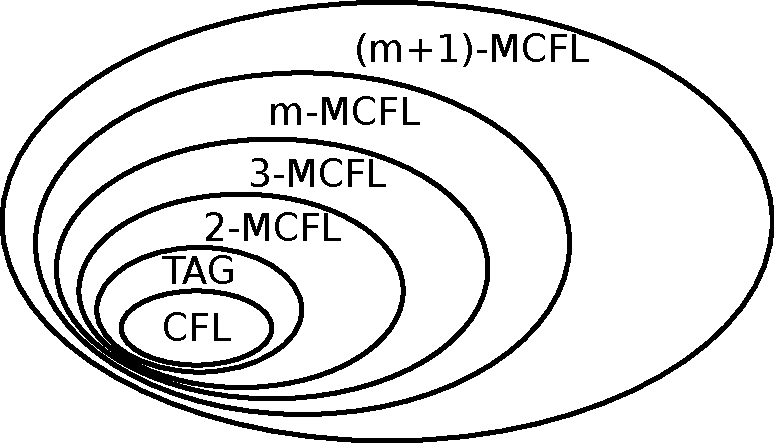
\includegraphics[width=\textwidth]{pics/mcfg.pdf}
\end{frame}

\begin{frame}[fragile]

 \frametitle{Иерархия для $m=1$}
 \begin{rutheorem}
  1-MCFL = CFL
 \end{rutheorem}
\pause
 \begin{rutheorem}
  1-MCFL(1) $\varsubsetneq$ 1-MCFL(2)
 \end{rutheorem}
 \pause
 \begin{rutheorem}
  1-MCFL($r$) = 1-MCFL($r+1$), $r\geq2$
 \end{rutheorem}

\end{frame}


\begin{frame}[fragile]

 \frametitle{Иерархия для $m=2$}
 \begin{rutheorem}[Ramow, Satta]
  2-MCFL(2) = 2-MCFL(3)
 \end{rutheorem}

 \begin{rutheorem}
 Если $m>2$ или $r>2$, то m-MCFL(r) $\varsubsetneq$ m-MCFL(r+1)
 \end{rutheorem}

\end{frame}


\begin{frame}[fragile]

  \frametitle{Иерархия по $r$}

  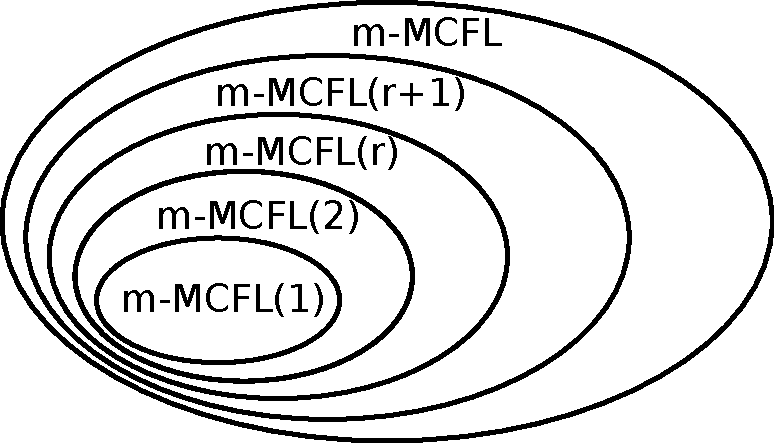
\includegraphics[width=\textwidth]{pics/mcfg_2.pdf}

\end{frame}


\begin{frame}[fragile]

  \frametitle{$MIX$}
  \begin{itemize}
    \item $mix = \{\omega \in \{a,b\}^* \mid |\omega|_a = |\omega|_b \}$ --- контекстно-свободный язык

    \item $MIX = \{\omega \in \{a,b,c\}^* \mid |\omega|_a = |\omega|_b = |\omega|_c\}$ --- MCFL? Хотелось верить, что нет
    \begin{itemize}
      \item \href{https://hal.inria.fr/inria-00564552/document}{MIX is a 2-MCFL and the word problem in $\mathbb{Z}^2$ is solvedby a third-order collapsible pushdown automaton, Sylvain Salvati, 2011}
    \end{itemize}
    \pause
    \item $O_2=\{\omega \in \{a,\overline{a},b,\overline{b}\}^* \mid |\omega|_a=|\omega|_{\overline{a}} \wedge |w|_b=|w|_{\overline{b}}\}$

    \item $O_n=\{\omega \in \{a_1,\overline{a_1},a_2,\overline{a_2},\ldots,a_n,\overline{a_n}\}^* \mid |\omega|_{a_1}=|\omega|_{\overline{a_1}} \wedge |w|_{a_2}=|w|_{\overline{a_2}} \wedge \cdots \wedge |w|_{a_n}=|w|_{\overline{a_n}}\}$
    \item $MIX_n = \{\omega \in \{a_1,\ldots,a_n\}^* \mid |\omega|_{a_1} = |\omega|_{a_2} =\cdots = |\omega|_{a_n}\}$
    \pause
    \item $MIX_n$ регулярно эквивалентен $O_n$ (существует алгоритм построения грамматики одного языка по грамматике другого)
    \begin{itemize}
      \item \href{https://hal.archives-ouvertes.fr/hal-01771670/document}{$O_n$ is an n-MCFL, Sylvain Salvati, 2018}
    \end{itemize}
  \end{itemize}
\end{frame}


\begin{frame}[fragile]

  \frametitle{Направления развития}

  \begin{itemize}
    \item Уточнение внутренних иерархий
    \item Сопоставление с другими классами и иерархиями
    \item Представимость языков
    \begin{itemize}
      \item Ваианты леммы о накачке
      \item Представимость конкретных языков
      \begin{itemize}
        \item Многомерный язык Дика: \href{https://link.springer.com/chapter/10.1007/978-3-662-59620-3_5}{Towards a 2-Multiple Context-Free Grammar for the 3-Dimensional Dyck Language, Konstantinos Kogkalidis, Orestis Melkonian, 2019}
        \item Шафл языков Дика: \href{https://dl.acm.org/doi/10.1145/3093333.3009848}{Context-sensitive data-dependence analysis via linear conjunctive language reachability, Qirun Zhang, Zhendong Su et al, 2017}
      \end{itemize}
    \end{itemize}
  \end{itemize}

\end{frame}

\begin{frame}[fragile]

  \frametitle{Граммтики и искуственные нейронные сети}

\begin{itemize}
    \item Учёт синтаксической структуры при синтезе: \href{https://dl.acm.org/doi/10.5555/3305381.3305582}{Grammar variational autoencoder, Kusner M. J., Paige B., Hernandez-Lobato J. M., 2017}
    \item Восстановление синтаксической структуры: \href{https://arxiv.org/abs/1804.06610}{End-to-end Graph-based TAG Parsing with Neural Networks, Jungo Kasai, Robert Frank et al, 2018}
    \item Извлечение грамматик: \href{https://link.springer.com/chapter/10.1007/978-3-662-48395-4_6}{Distributional Learning of Context-Free and Multiple Context-Free Grammars, Alexander Clark, Ryo Yoshinaka, 2019}
  \end{itemize}


\end{frame}


\end{document}
